~\label{chap:intro}
\begin{chapterabstract}
This introductory chapter outlines the motivation and background of this thesis, as well as it's objectives 
and structure.
\end{chapterabstract}

In recent years there has been much research activity in the field of 3D computer vision, a field concerned 
with the processing of three dimensional, geometric data for machine vision. This work addresses a number of 
open technical challenges within the field of active, 3D vision. Specifically, the 3D reconstruction of 
dynamic environments, robust 3D reconstruction of arbitrary objects and the prediction of shape \& pose of 
objects. These areas of research are of interest to the computer vision community due to the broad application 
potential of such systems. Scene reconstruction for example, has applications ranging from mobile robotics to 
recreating the tangible world for Virtual Reality (VR) viewing. Object reconstruction has applications including 
the reproduction of tangible objects via 3D printing and building 3D object models for the training of machine 
learning systems. Finally, shape and pose prediction allows representations of a machines environment to be 
inferred when traditional methods of reconstruction may not be feasible.

\section{3D Scene Reconstruction and Understanding}
~\label{sec:intro_scene_recon}
Driven by the availability of consumer grade depth sensing equipment such as the Microsoft Kinect RGBD camera 
(introduced by Microsoft for the XBox 360), there has been a renewed interest in dense scene reconstruction. 
Advances in recent years have allowed for the creation of digital reconstructions of the tangible world with 
consumer grade computer equipment. Such systems iteratively integrate observed world points into a ``global'' 
model, such that over time, a smooth representation of the observed world surfaces is built. In addition to the 
integration of such information into a model, there is the task of inferring how the sensor has moved in world 
space, such that the observed points may be transformed and integrated into the appropriate model location. The 
amalgamation of these two tasks is known as SLAM (Simultaneous Localisation and Mapping). A typical 
reconstruction using such a system is given in Figure~\ref{figure:room_recon_example}.
\begin{figure}[!htbp]
  \centering
  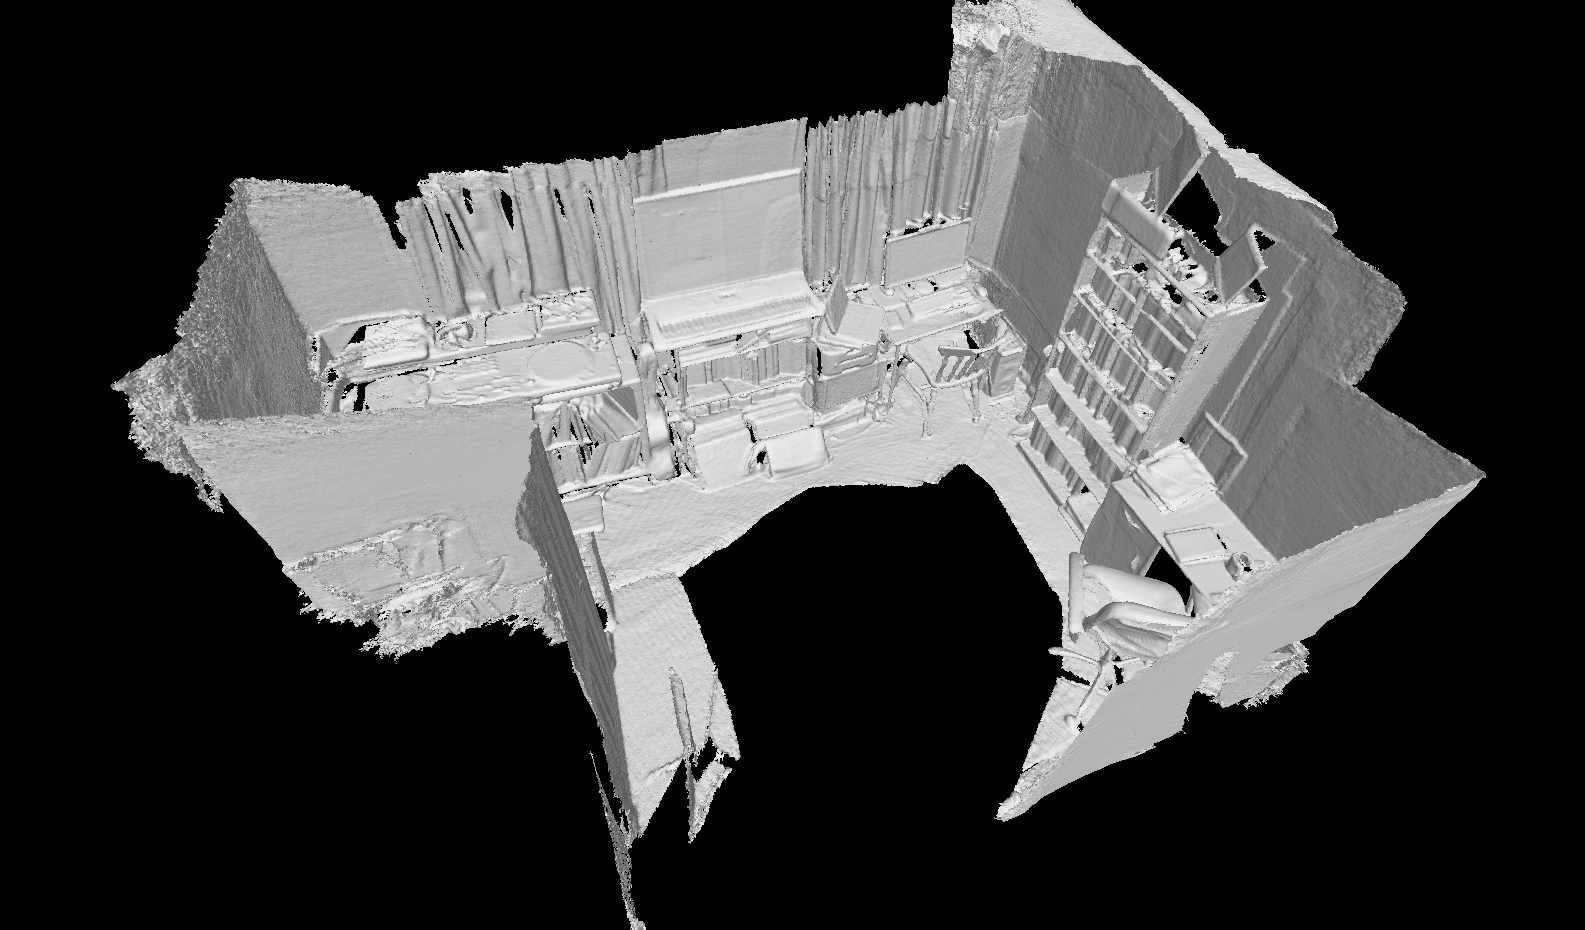
\includegraphics[width=.7\linewidth]{figures/intro/room_scene.png}
  \caption[Room Scale Dense Reconstruction]{An example of room-scale dense reconstruction.}
~\label{figure:room_recon_example}
\end{figure}
% TODO: SLAM pipeline figure

There has been much advancement in the 2D semantic scene understanding literature, which can be utilised within 
the context of 3D vision to introduce a semantic component to dense SLAM systems. Such a combination of techniques 
provides an adaptable component to AR and robotics applications. Early work on amalgamating the two areas of research 
have allowed one to view a reconstruction of their environment in VR and interactively label some of the objects within 
it, with the system inferring the remaining labellings. An example of the output of such a system is given 
in Figure~\ref{figure:spaint_teaser}.
\afterpage{
  \begin{figure}[!htbp]
    \centering
    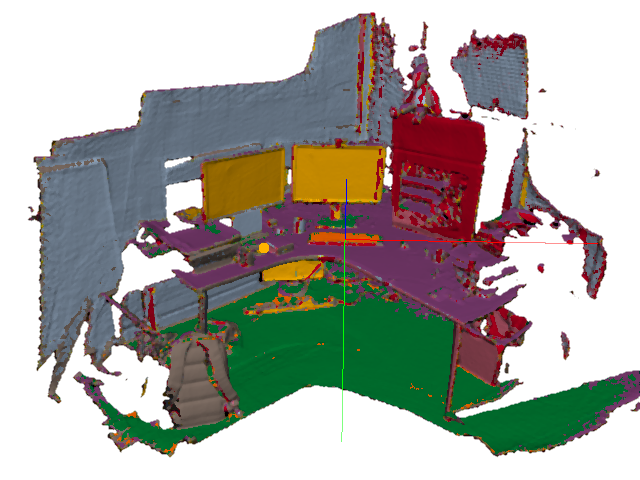
\includegraphics[width=.7\linewidth]{figures/intro/spaint-teaser.png}
    \caption[Room Scale Dense Reconstruction]{An example of semantic SLAM.\footnotemark}
~\label{figure:spaint_teaser}
  \end{figure}
~\footnotetext{Copyright \textit{Golodetz et al}, 2015.\\
\url{http://www.robots.ox.ac.uk/~tvg/projects/SemanticPaint/index.php}}
}

Though the results of the systems shown in Figures~\ref{figure:room_recon_example} and~\ref{figure:spaint_teaser} 
represent impressive advancements in computer vision, there are however open technical challenges. One such 
challenge is the successful modelling of real environments in which there are dynamic components (such as 
people walking in the camera's view). The traditional dense SLAM pipeline is unable to accurately build a 
globally consistent model in such environments. In addition, when using a combined reconstruction and 
semantics system such as that shown in Figure~\ref{figure:spaint_teaser}, many of the descriptive cues that 
enable the segmentation to be performed rely on features utilising 2D image information. As such, there is 
no ``true'' semantic 3D object learning and recognition.

As outlined, traditional dense SLAM systems have difficulty performing dense reconstruction in an 
environment where there is motion. The aforementioned sensor pose estimation phase in many such systems
is prone to error or failure in such a scenario. The reason for this is due to the reliance on point based 
correspondences between frames. If a static environment is being modelled, then a high number of valid point 
correspondences will be found. However, when motion (independent of the sensors motion) is introduced into 
the scene, invalid correspondences may be found. For example, points that belong to a non moving object 
such as a chair may erroneously be matched to those on a moving scene component, such as a walking person.
Such erroneous correspondences can incur failure cases ranging from moderate model inconsistencies to total 
loss of sensor tracking.

Though there are many use cases for static scene reconstruction, the lack of robustness to dynamics is 
prohibitive in scenarios where a high level of machine perception is required. For example, if 
reconstructing a busy working environment in which there is a high level of dynamics (people walking, 
doors opening etc), an ideal reconstruction would not include artifacts of such motion. As such, the 
reconstruction system would be required to identify such components and account for them in the 
reconstruction process. Additionally, a system that is capable of detecting and segmenting such motion 
would be capable of extracting pertinent semantic information from such events.

\section{Object Reconstruction}
~\label{sec:intro_object_recon}
Modern machine learning provides much of the semantic and contextual information required to make meaningful 
inferences over the state of the world, as observed by a sensor (such as a camera). Much advancement 
has been made in recent years on the tasks of object detection and semantic segmentation, in standard 2D 
images. However, there are many technical challenges that must be overcome before such efficacy on these 
tasks is reached for the 3D case. Many modern AI and machine learning algorithms require vast quantities of 
data to learn to perform a given task successfully. This is not prohibitive for systems that operate on standard 
2D images, due to the abundance of available data. However, for the 3D case there is not a comparable volume of 
3D data with real world geometric information from which a system can learn to perform complex tasks in the real 
world. One method of obtaining such geometric data is the reconstruction of objects, providing geometrically 
accurate models of real world objects.
% TODO: object reconstruction figure.

A related problem to that of sensor pose estimation as outlined in Section~\ref{sec:intro_scene_recon}, 
is pose estimation when performing reconstruction of individual objects. As with the larger scale case, point 
correspondences are problematic. One prominent reason is that for a smaller object versus a full scale scene 
(such as a room), there is less geometric data available in the former case than in the latter. As with the larger 
scale reconstruction, inconsistencies in the pose estimation phase can have varying effects on the resultant 
reconstruction. Such inconsistencies in the reconstruction can have a detrimental effect on learning based systems 
for 3D tasks if such inconsistent reconstructions are used to train such models. This is particularly troublesome as 
inconsistencies in object scale models in some cases have a more pronounced effect than in the case where 
an entire room is being reconstructed.

Though the model consistency problem for objects may be circumvented somewhat when using specialist equipment 
such as modelling turntables and laser range scanners, there are financial and practical issues that can be 
prohibitive. Thus, the ability to build high quality, consistent reconstructions of arbitrary objects with 
commodity depth sensing and computing hardware is desirable.

\section{Shape Prediction and Pose Prediction}
~\label{sec:intro_spp}
Though for many reconstruction scenarios the approaches outlined in Sections~\ref{sec:intro_scene_recon} 
and~\ref{subsec:intro_object_recon} are applicable, there are some situations in which the aforementioned 
approaches are not practical. For a complete, closed model, the reconstruction based approaches require that 
the object be fully observable, such that full coverage with the depth sensor is possible. As such, a clear 
failure point is the case in which the object is not fully observable, for example, when reconstructing a large 
object that is on a wall.

Additionally, the scene and object reconstruction approaches previously outlined depend on the iterative 
integration of observed range data. This approach may be troublesome in a scenario where an object may not 
be visible to the sensor for a sufficient period of time to build a smoothly reconstructed model. Circumventing 
this issue would require a very high framerate sensor. Additionally, the highly dynamic nature of such a scenario 
is likely to be problematic in a similar manner to outlined case of dynamic dense SLAM\@.

As such, a desirable approach to the 3D modelling of objects in problematic environments would not rely on 
direct reconstruction (in the sense of the integration of range data into a 3D model). Rather, an inference based 
approach is appropriate, due to the inherent stochastisity of building a full model of a partially observable 
object.

\section{Technical Aims and Thesis Structure}
~\label{sec:intro_aims_structure}
The aforementioned technical challenges pertain to the dense reconstruction of dynamic scenes, the 
reconstruction of objects and the reconstruction of objects for which no full view is available. As 
such, the following main research challenges are addressed in this work.
\begin{itemize}
  \item The dense reconstruction of dynamic environments.
  \begin{itemize}
    \item With real time performance.
    \item With comparable reconstruction quality to static counterpart.
    \item With an improvement in pose estimation over static counterpart.
  \end{itemize}
  \item Identifying the dynamic components of a scene.
  \begin{itemize}
    \item Utilising for semantics.
  \end{itemize}
  \item The reconstruction of arbitrary objects in a consistent manner.
  \begin{itemize}
    \item With comparable reconstruction quality to scene based alternative.
    \item With commodity hardware for wider applicability.
    \item Without known pose.
  \end{itemize}
  \item The inference of object centric scene properties where traditional reconstruction 
may not be possible.
  \begin{itemize}
    \item Inferring both shape and pose.
    \item Without requiring temporally consistent frames, averting tracking errors.
  \end{itemize}
\end{itemize}

With the central technical challenges of this work outlined, the remainder of this work is structured 
as follows. Firstly, Chapter~\ref{chap:lit_review} provides a comprehensive survey of the literature 
pertinent to this work. Initially, a survey of the dense SLAM (as introduced earlier in this chapter) 
literature is provided. The research outlined in this section is fundamental to much of the content of 
this work. Additionally, relevant works on semantics (such as semantic SLAM) are reviewed. 
Next in Chapter~\ref{chap:lit_review} is an assessment of relevant research on the topic of dynamics in 
3D vision; topics include motion segmentation, optical and scene flow. Much of the material reviewed in 
this section is pertinent to the subject matter of Chapter~\ref{chap:moseg}. The next major area of 
research to be reviewed is on the topic of object reconstruction; relevant background to the topic of 
Chapter~\ref{chap:probobj}. Finally, Chapter~\ref{chap:lit_review} concludes with an assessment of the 
literature on the topics of pose prediction and shape prediction.

Chapter~\ref{chap:moseg} introduces the approach taken in this work to the problem of dense reconstruction 
in dynamic environments (environments with moving components). The chapter begins by outlining fundamental 
concepts in the static dense SLAM pipeline that shall be fundamental to much of the content in this work. 
Following this fundamental material, an approach to peforming dense reconstruction and motion segmentation 
in dynamic scenes is presented. The method outlined in this chapter is evaluated against a state of the art 
dense SLAM system for static scenes, to which the presented approach demonstrates an overall improvement 
versus the static dense SLAM system. Additionally, the qualitative results of the presented approach 
demonstrate high quality resultant reconstructions on the test scenes. Furthermore, Chapter~\ref{chap:moseg} 
provides a demonstration of utilising motion segmentation to perform rudementary object recognition using 
3D geometric features.

Chapter~\ref{chap:probobj} introduces a novel approach to the segmentation and reconstruction of individual 
objects. The chapter outlines a novel Probabilistic approach to object reconstruction that reduces 
inconsistencies in pose estimation, which positively impacts the overall reconstruction quality. The 
approach presented in this chapter works with commodity computer and depth sensing equipment (though in 
principle it is trivially extendable, by design) and yields high quality reconstructions. Reconstruction 
quality is evaluated quantitatively and qualitatively against multiple alternative approaches. A 
quantitative evaluation of pose estimation quality is also provided, demonstrating an improvement over 
alternative approaches. The work in this chapter has been peer reviewed and published in the 
\textit{International Conference on 3D Vision (3DV)}.

% -- "Stereo Shape and Pose Regression"
% ---- Outline approach; which questions adressed?
% ---- Outline experiments
% ---- Outline results
Chapter~\ref{chap:spp} approaches the problem of performing inference of shape and pose simultaneously. 
The work in this chapter is notably different in nature relative to the approaches taken in Chapters
~\ref{chap:moseg} and~\ref{chap:probobj}; Chapter~\ref{chap:spp} utilises a data driven, non SLAM based 
approach to learn predictive models for shape and pose in a semi-supervised manner. A full view of the 
object of interest is not required, nor is temporal consistency between frames; ad-hoc prediction can be 
performed for arbitrarily sequenced frames.